\chapter{Avaliação e Validação}
\label{ch:avaliacao}

\section{Prova de Conceito – Avaliação da Proposta}
\label{sc:provaConceito}

Com a finalidade de verificar se os objetivos que foram especificados neste trabalho, realmente, foram atingidos com o desenvolvimento do aplicativo apresentado, foi realizado uma prova de conceito. O intuito da prova de conceito é criar um modelo prático que possa provar o conceito estabelecido por uma pesquisa ou artigo técnico, isto é, não se faz necessário que o experimento esteja totalmente finalizado, mas que permita demonstrar como o mesmo pode contribuir para a colaboração, bem como a produção de conhecimento \cite{tornela07}.

A prova de conceito foi realizada no período de 11 a 13 de novembro de 2014 e consistiu na elaboração de um questionário de avaliação da versão 1.0.5  do aplicativo FindBus \footnote{https://itunes.apple.com/br/app/findbus/id775452035?mt=8}, lançada em março de 2014 e disponível na App Store, loja de aplicativo da Apple, bem como da versão 1.0.1 lançado em setembro de 2015 na Google Play \footnote{https://play.google.com/store/apps/details?id=br.com.altcompany.findbus}, loja de aplicativo da Google. 

O questionário de avaliação conteve 25 questões e foi dividido em duas etapas: etapa de reconhecimento e etapa de avaliação. A primeira teve como objetivo reconhecer o perfil do usuário, bem como verificar se o mesmo estaria apto a avaliar o aplicativo. A segunda etapa consistiu em 22 perguntas diretamente relacionadas ao uso da aplicação, objetivando, assim, realmente avaliar se a proposta está funcionando conforme fora especificada. 

O questionário de avaliação foi enviado para o e-mail de 3000 usuários, todos eles com mais de 3 meses de uso. Nesse ínterim, foi possível coletar 63 respostas para o questionário e, como base nelas, os resultados da realização da prova de conceito foram expressos na seção subsequente. 

\section{Apresentação dos resultados}
\label{sc:apresentacaoResultados}

O questionário foi desenvolvido com base nos objetivos descritos na seção \ref{sc:objetivo} deste trabalho, onde o principal objetivo foi, exatamente, certificar-se de que a proposta desenvolvida atendia todos os objetivos apresentados. Para tanto, conforme mencionado no início desta seção, criou-se um questionário utilizando o Google Forms, ferramenta da Google para criação de formulários, contendo 25 questões. A referida pesquisa ficou disponível por um período de três dias e foi possível obter, nesse ínterim, 63 respostas para a mesma.  

A ideia da pesquisa de avaliação não foi analisar os dados fornecidos de forma individual, mas sim segmentá-los apenas para análise estatística. A participação foi voluntária e, como nenhum participante precisou se identificar, os dados foram anônimos e confidenciais.    

Doravante os dados das principais perguntas serão apresentados obedecendo a seguinte estrutura: questão; apresentação dos dados em uma tabela e, quando necessário, apresentação dos dados em um gráfico; breve comentário sobre os resultados, isto é, uma análise parcial dos dados.

\textbf{Questão 1:  Qual plataforma você está utilizando?}

\begin{center}
\begin{longtable}{c|c|c}
\hline
    \multicolumn{1}{c}{\textbf{Resultado}} & \multicolumn{1}{c}{\textbf{Quantidade}} & \multicolumn{1}{c}{\textbf{Percentual}} \\
\hline
    IOS & 47 &  75\%\\
    \hline
    Android & 16 & 25\%\\
    \hline
\caption{Tabela de resultados obtidos na questão 1}
\end{longtable}
\end{center}


\begin{figure}[h]
\begin{center}
  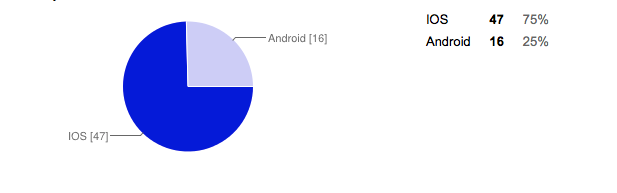
\includegraphics[width=7cm]{images/graficos/questao1.png}
  \caption{Gráfico de resultados da questão 1}
  \label{fig:questao1}
\end{center}
\end{figure}

\textbf{Comentários:}

O objetivo dessa pergunta foi avaliar se os objetivos descritos neste trabalho foram atendidos para todas as plataformas para quais a proposta foi desenvolvida. Não obstante, como as respostas foram bastante similares para ambas plataformas, os dados não foram analisados separadamente. 

Observa-se que 75\% dos usuários que participaram da pesquisa utilizam a ferramenta desenvolvida para plataforma IOS, enquanto que 25\% utilizam a plataforma Android.\newline

\textbf{Questão 2: Ao logar no aplicativo, o sistema conseguiu identificar a cidade onde você se encontra?}

\begin{center}
\begin{longtable}{c|c|c}
\hline
    \multicolumn{1}{c}{\textbf{Resultado}} & \multicolumn{1}{c}{\textbf{Quantidade}} & \multicolumn{1}{c}{\textbf{Percentual}} \\
\hline
    Sim & 61 &  97\%\\
    \hline
    Não & 2 & 3\%\\
    \hline
\caption{Tabela de resultados obtidos na questão 2}
\end{longtable}
\end{center}


\begin{figure}[h]
\begin{center}
  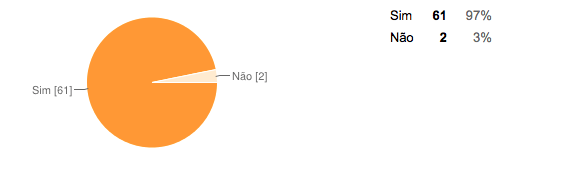
\includegraphics[width=15cm]{images/graficos/questao2.png}
  \caption{Gráfico de resultados da questão 2}
  \label{fig:questao1}
\end{center}
\end{figure}

\textbf{Comentários:}

O objetivo dessa pergunta foi avaliar a sensibilidade ao contexto existente na aplicação, pois se a mesma consegue identificar a cidade, ou seja, o contexto de localização que o usuário se encontra, ela consegue encaixar o usuário no contexto correto, em outras palavras, dessa forma, é possível mostrar para os usuários todos os ônibus, linhas, pontos, incidentes, bem como todas as informações no tocante a sua cidade.
	
Observa-se, através do gráfico mostrado na figura \figref{fig:questao1}, que 97\% dos usuários afirmaram que realmente o sistema consegue identificar em qual cidade o usuário se encontra, enquanto que, apenas, 3\% afirmaram o contrário. 

\textbf{Questão 3:  Você se encontra em uma cidade atendida pelo aplicativo (São Paulo, Curitiba, New York e Boston)?}

\begin{center}
\begin{longtable}{c|c|c}
\hline
    \multicolumn{1}{c}{\textbf{Resultado}} & \multicolumn{1}{c}{\textbf{Quantidade}} & \multicolumn{1}{c}{\textbf{Percentual}} \\
\hline
    Sim & 44 &  70\%\\
    \hline
    Não & 19 & 30\%\\
    \hline
\caption{Tabela de resultados obtidos na questão 3}
\end{longtable}
\end{center}


\begin{figure}[h]
\begin{center}
  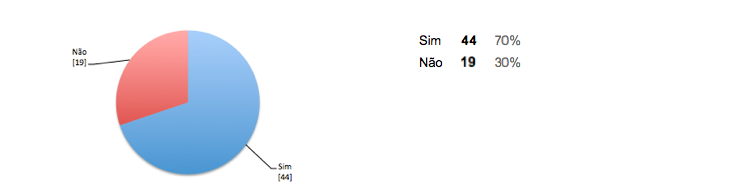
\includegraphics[width=16cm]{images/graficos/questao3.png}
  \caption{Gráfico de resultados da questão 3}
  \label{fig:questao3}
\end{center}
\end{figure}

\textbf{Comentários:}

Atualmente, o aplicativo está funcionando nas cidades de São Paulo, Curitiba, Boston e New York. Portanto, somente os usuários que utilizam o aplicativo em umas dessas cidades possuem condições de avaliar todas as funcionalidades contidas no mesmo. Isto posto, o principal objetivo da pergunta foi exatamente identificar as pessoas que  poderiam prosseguir para segunda etapa do questionário, a etapa de avaliação. 
	
Observa-se que 44 pessoas, do universo de 63 usuários, que responderam o questionário estavam em uma das cidades atendidas pelo aplicativo, o que representa um total de 70\% do total de entrevistados. Nota-se que, como a pergunta determinava o fim ou o prosseguimento do questionário, apenas 44 pessoas deram continuidade e passaram para etapa de avaliação, o que significa dizer o que a partir da próxima pergunta o número de respostas passará de 63 para 44, sendo assim, tivemos na etapa de avaliação 70\% das pessoas que se propuseram a responder o questionário.\newline

\textbf{Questão 4: Ao logar, você é direcionado para tela principal do sistema. Nessa tela, você consegue visualizar os ônibus que estão perto de sua localização?}

\begin{center}
\begin{longtable}{c|c|c}
\hline
    \multicolumn{1}{c}{\textbf{Resultado}} & \multicolumn{1}{c}{\textbf{Quantidade}} & \multicolumn{1}{c}{\textbf{Percentual}} \\
\hline
    Sim & 40 &  63\%\\
    \hline
    Não & 04 & 6\%\\
    \hline
\caption{Tabela de resultados obtidos na questão 4}
\label{tabq4}
\end{longtable}
\end{center}


\begin{figure}[h]
\begin{center}
  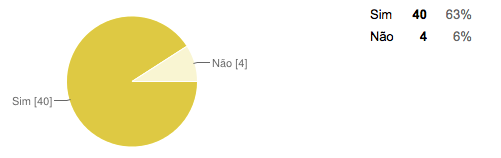
\includegraphics[width=16cm]{images/graficos/questao4.png}
  \caption{Gráfico de resultados da questão 4}
  \label{fig:questao4}
\end{center}
\end{figure}

\textbf{Comentários:}

Algumas das perguntas criadas no questionário de avaliação tiveram o objetivo de guiar o usuário, apresentar a aplicação, bem como garantir que o usuário realmente utilizou o aplicativo. Deste modo, fazendo com que os dados colhidos, sobretudo nas questões cuja finalidade é validar os objetivos propostos neste trabalho, sejam fidedignos. Não obstante, os dados coletados nessa questão comprovam, conforme pode ser visto no gráfico da figura  \figref{fig:questao4} e na tabela \ref{tabq4}, o quão o aplicativo se preocupa com a localização do usuário, em mostrar o que está acontecendo ao seu redor.\newline

\textbf{Questão 5: Ao clicar em um determinado ônibus, o nível de informação mostrada pelo aplicativo é suficiente (linha, identificação do ônibus, tempo de atualização, distância, endereço)?}

\begin{center}
\begin{longtable}{c|p{1cm}|p{1cm}|p{2cm}|p{1cm}|p{1cm}}
\hline
    \multicolumn{1}{c}{\textbf{Item/Opção}} & \multicolumn{1}{c}{\textbf{DT}} & \multicolumn{1}{c}{\textbf{D}} & \multicolumn{1}{c}{\textbf{ND,NC}} & \multicolumn{1}{c}{\textbf{C}} & \multicolumn{1}{c}{\textbf{CT}} \\
\hline
    Identificação da linha & 1 & 0 & 1 & 26 & 16\\
    \hline
    Identificação do ônibus & 1 & 0 & 2 & 26 & 15\\
    \hline
     Tempo de atualização & 1 & 0 & 11 & 20 & 6\\
    \hline
    Distância & 2 & 5 & 5 & 27 & 5\\
    \hline
     Endereço & 1 & 0 & 2 & 28 & 13\\
     \hline
\caption{Tabela de resultados obtidos na questão 4}
\label{tabq5}
\end{longtable}
\end{center}

Legenda: DT = Discordo totalmente; D = Discordo; ND,NC = Nem discordo, nem concordo; C = Concordo; CT = Concordo totalmente.

\textbf{Comentários:}

O aplicativo se propõe a munir o usuário com o máximo de informação no tocante ao meio de transporte público que o mesmo comumente utilize, aumentando, dessa forma, o poder de decisão deste. Isto posto, com a finalidade de medir a qualidade, bem como a satisfação do usuário para com o nível de informação disponibilizada pelo aplicativo, a pergunta 5 teve como objetivo validar se as informações mostradas referentes a identificação da linha, identificação do ônibus, tempo de atualização do veículo, distância do veículo para o usuário e endereço onde o ônibus se encontra são realmente suficientes.
	
Analisando os dados disponíveis na tabela \ref{tabq5}, observa-se, de modo geral, que a maioria das pessoas que se propuseram a responder o questionário concordaram que o nível de informação mostrada no que tange aos ônibus é satisfatória. Contudo, vale ressaltar que quando se refere ao tempo de atualização o nível de satisfação não é tão bom como acontece com os outros itens avaliados na questão.\newline

\textbf{Questão 6: Na tela principal, ao tentar digitar o nome ou número de uma linha, você consegue encontrar todas as linhas existentes em sua cidade.}

\begin{center}
\begin{longtable}{c|c|c}
\hline
    \multicolumn{1}{c}{\textbf{Resultado}} & \multicolumn{1}{c}{\textbf{Quantidade}} & \multicolumn{1}{c}{\textbf{Percentual}} \\
\hline
    Concordo totalmente & 28 &  44\%\\
    \hline
    Concordo parcialmente & 14 & 22\%\\
    \hline
     Não concordo & 2 & 3\%\\
    \hline
\caption{Tabela de resultados obtidos na questão 6}
\label{tabq6}
\end{longtable}
\end{center}


\begin{figure}[h]
\begin{center}
  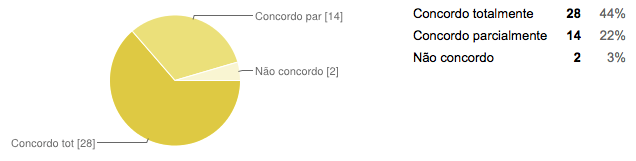
\includegraphics[width=16cm]{images/graficos/questao6.png}
  \caption{Gráfico de resultados da questão 6}
  \label{fig:questao6}
\end{center}
\end{figure}

\textbf{Comentários:}

Uma dos requisitos do aplicativo é exatamente fazer com que o usuário saiba todas as linhas existente na cidade que ele se encontra. Isto posto, a questão 6 foi criada com a finalidade de validar se realmente a aplicação atende tal requisito. 
	
Observa-se que 42 pessoas, do total de 44, concordam que o aplicativo consegue mostrar todas as linhas existente na cidade do usuário, enquanto que, apenas, 2 pessoas afirmaram o contrário. Nesse sentido, de maneira geral, analisando os dados apresentados no gráfico presente na figura \figref{fig:questao6}, nota-se que o aplicativo consegue, na maioria das vezes, mostrar aos seus usuários todas as linhas existentes na cidades em que estes se encontram.\newline

\textbf{Questão 7: Na aba de ocorrências, você consegue visualizar a ocorrência cadastrada, bem como quais linhas estão sendo afetadas pelo incidente informado?}

\begin{center}
\begin{longtable}{c|c|c}
\hline
    \multicolumn{1}{c}{\textbf{Resultado}} & \multicolumn{1}{c}{\textbf{Quantidade}} & \multicolumn{1}{c}{\textbf{Percentual}} \\
\hline
    Sim & 41 &  65\%\\
    \hline
    Não & 3 & 5\%\\
    \hline
\caption{Tabela de resultados obtidos na questão 7}
\label{tabq7}
\end{longtable}
\end{center}


\begin{figure}[h]
\begin{center}
  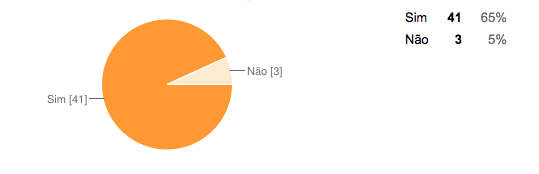
\includegraphics[width=16cm]{images/graficos/questao7.png}
  \caption{Gráfico de resultados da questão 7}
  \label{fig:questao7}
\end{center}
\end{figure}

\textbf{Comentários:}

A questão 7 tem como objetivo atestar se os usuários conseguem cadastrar ocorrências de incidentes de trânsito, sobretudo, se estes conseguem saber quais linhas estão sendo afetadas por tais eventos, exatamente como fora proposto nos objetivos deste trabalho.
	
Nota-se, analisando os dados apresentados, que a maioria das avaliações foram positivas, onde a maioria das pessoas conseguiram tanto cadastrar os incidentes vivenciados, como visualizar quais linhas o incidente estava afetando. \newline

\textbf{Questão 8: Na aba de destino, ao tentar encontrar as linhas que te levará até o destino informado, como você classifica a recomendação feita pelo aplicativo? }

\begin{center}
\begin{longtable}{c|c|c}
\hline
    \multicolumn{1}{c}{\textbf{Resultado}} & \multicolumn{1}{c}{\textbf{Quantidade}} & \multicolumn{1}{c}{\textbf{Percentual}} \\
\hline
    1 & 2 &  3\%\\
    \hline
    2 & 1 & 2\%\\
    \hline
    3 & 3 &  5\%\\
    \hline
    4 & 27 & 43\%\\
    \hline
    5 & 11 & 17\%\\
    \hline
\caption{Tabela de resultados obtidos na questão 8}
\label{tabq8}
\end{longtable}
\end{center}


\begin{figure}[h]
\begin{center}
  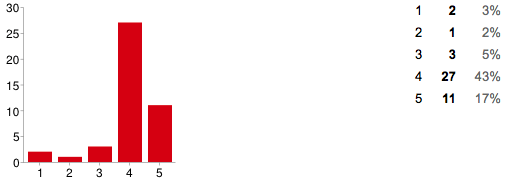
\includegraphics[width=16cm]{images/graficos/questao8.png}
  \caption{Gráfico de resultados da questão 8}
  \label{fig:questao8}
\end{center}
\end{figure}

\textbf{Comentários:}

Uma das funcionalidades que este trabalho propusera fornecer ao usuário é a recomendação de linhas, onde o mesmo conseguiria saber qual linha o levaria à um determinado destino a partir de um determinado ponto. Isto posto, a questão 8 tem o objetivo de validar se as linhas recomendadas pelo aplicativo realmente  servem para os usuários  chegarem até seus destinos. Para tanto, pediu-se aos participantes da avaliação que classificassem a recomendação feita pelo aplicativo com uma nota de 1 a 5, onde 1 representava uma total insatisfação e 5 uma total satisfação com a recomendação.

No gráfico mostrado na figura \figref{fig:questao8}, é possível observar uma concentração maior nas opções de classificação 4 e 5, o que comprova que a maioria dos participantes ficaram satisfeitos com a recomendação feita pelo aplicativo. Vale destacar que a satisfação não foi unanimidade, tendo, portanto, 3 avaliações, de um total  de 44, totalmente negativas. \newline

\textbf{Questão 9: Como você classifica o nível de informação disponibilizada pelo aplicativo?}

\begin{center}
\begin{longtable}{c|c|c}
\hline
    \multicolumn{1}{c}{\textbf{Resultado}} & \multicolumn{1}{c}{\textbf{Quantidade}} & \multicolumn{1}{c}{\textbf{Percentual}} \\
\hline
    1 & 3 &  5\%\\
    \hline
    2 & 1 & 2\%\\
    \hline
    3 & 2 &  3\%\\
    \hline
    4 & 29 & 46\%\\
    \hline
    5 & 9 & 9\%\\
    \hline
\caption{Tabela de resultados obtidos na questão 9}
\label{tabq9}
\end{longtable}
\end{center}


\begin{figure}[h]
\begin{center}
  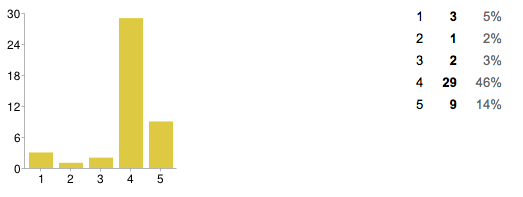
\includegraphics[width=16cm]{images/graficos/questao9.png}
  \caption{Gráfico de resultados da questão 9}
  \label{fig:questao9}
\end{center}
\end{figure}

\textbf{Comentários:}

O aplicativo se propõe a fornecer uma grande quantidade de informação à seus usuários, todavia, é necessário que se saiba o nível da informação disponibilizada. Para tanto, a questão 9 pediu para que os participantes da avaliação classificassem o nível de informação disponibilizada pelo aplicativo com uma nota no intervalo de 1 a 5, onde 1 significava dizer que o sistema fornecia um péssimo nível de informação, enquanto que 5 significava que o usuário considerava o nível de informação disponibilizada pelo aplicativo excelente. 
	
Análogo ao que aconteceu na questão 8, analisando o gráfico da figura \figref{fig:questao9}, observa-se uma concentração maior nas respostas 4 e 5, o que valida a satisfação da maioria dos usuários no que tange o nível de informação disponibilizada pela aplicação. \newline

\textbf{Questão 10: A utilização do FindBus ajuda a otimizar o tempo?}

\begin{center}
\begin{longtable}{c|c|c}
\hline
    \multicolumn{1}{c}{\textbf{Resultado}} & \multicolumn{1}{c}{\textbf{Quantidade}} & \multicolumn{1}{c}{\textbf{Percentual}} \\
\hline
    Ajuda totalmente & 23 &  37\%\\
    \hline
    Ajuda parcialmente & 19 & 30\%\\
    \hline
    Não ajuda & 2 &  3\%\\
    \hline

\caption{Tabela de resultados obtidos na questão 10}
\label{tabq10}
\end{longtable}
\end{center}


\begin{figure}[h]
\begin{center}
  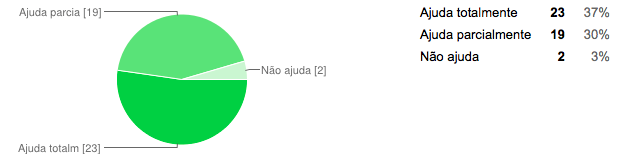
\includegraphics[width=16cm]{images/graficos/questao10.png}
  \caption{Gráfico de resultados da questão 10}
  \label{fig:questao10}
\end{center}
\end{figure}

\textbf{Comentários:}

Uma das grandes propostas do aplicativo proposto neste trabalho é fazer com que seus usuários possam otimizar o tempo ao utilizar os serviços de transporte público para se locomoverem. Portanto, a questão 10 foi criada com a finalidade de provar que o mesmo, realmente, consegue propiciar tal beneficio aos seus usuários. 
	
Analisando o gráfico ilustrado na figura \figref{fig:questao10}, nota-se que 42 pessoas, de um total de 44 avaliados, afirmaram que conseguem otimizar o tempo com a utilização do FindBus. Portanto, pode-se afirmar que com a utilização do aplicativo proposto neste trabalho é possível perder menos tempo ao se locomover pela cidade e, por conseguinte, aproveitar melhor o tempo disponível.\newline

\textbf{Questão 11: Como você classifica a localização e tempo de atualização da posição dos ônibus no aplicativo?}

\begin{center}
\begin{longtable}{c|c|c}
\hline
    \multicolumn{1}{c}{\textbf{Resultado}} & \multicolumn{1}{c}{\textbf{Quantidade}} & \multicolumn{1}{c}{\textbf{Percentual}} \\
\hline
    Muito ruim & 2 &  3\%\\
    \hline
    Ruim & 3 & 3\%\\
    \hline
    Aceitável & 12 &  19\%\\
    \hline
    Bom & 20 & 20\%\\
    \hline
    Muito bom & 7 & 7\%\\
    \hline
\caption{Tabela de resultados obtidos na questão 11}
\label{tabq11}
\end{longtable}
\end{center}

\begin{figure}[!h]
\begin{center}
  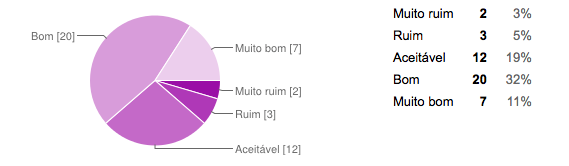
\includegraphics[width=14cm]{images/graficos/questao11.png}
  \caption{Gráfico de resultados da questão 11}
  \label{fig:questao11}
\end{center}
\end{figure}

\textbf{Comentários:}

Umas das grandes propostas do aplicativo foi fazer com que seus usuários pudessem acompanhar o deslocamento dos ônibus em, praticamente, tempo real. Com o intuito de avaliar se o aplicativo atende tal requisito, a questão 11 tem o propósito de mostrar se os usuários concordam com a localização dos ônibus mostrada no aplicativo, bem como com o intervalo de atualização da posição destes. 
	
Os dados mostrados na figura \figref{fig:questao11} revelam que, dos 44 usuários avaliados, 12 informaram que o tempo de atualização pode ser considerado aceitável, 20 acreditam que o tempo de atualização é bom e 7 consideram esse intervalo de tempo muito bom. Nesse sentido, conclui-se que a maioria dos participantes da pesquisa acharam que o intervalo de tempo de atualização é, no mínimo, aceitável.\newline

\textbf{Questão 12: A utilização do FindBus ajuda a estimar o exato momento que seu ônibus vai chegar no ponto?}

\begin{center}
\begin{longtable}{c|c|c}
\hline
    \multicolumn{1}{c}{\textbf{Resultado}} & \multicolumn{1}{c}{\textbf{Quantidade}} & \multicolumn{1}{c}{\textbf{Percentual}} \\
\hline
    Ajuda totalmente & 14 &  22\%\\
    \hline
    Ajuda parcialmente & 28 & 44\%\\
    \hline
    Não ajuda & 2 &  3\%\\
    \hline

\caption{Tabela de resultados obtidos na questão 12}
\label{tabq12}
\end{longtable}
\end{center}


\begin{figure}[h]
\begin{center}
  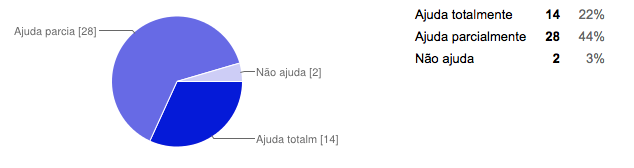
\includegraphics[width=15cm]{images/graficos/questao12.png}
  \caption{Gráfico de resultados da questão 12}
  \label{fig:questao12}
\end{center}
\end{figure}

\textbf{Comentários:}

Esta questão foi desenvolvida com a finalidade de atestar se o aplicativo fornece subsídios suficientes para que os usuários consigam estimar o exato momento que seu veículo chegará ao ponto de ônibus. 
Analisando os dados contidos na tabela X, observa-se que 22\% dos avaliados consideram que o aplicativo ajuda totalmente a prever o momento que o ônibus vai chegar no ponto, 44\% acreditam que o aplicativo ajuda, no entanto, de maneira parcial, enquanto que apenas 3\% informaram que o sistema não ajuda a fazer essa estimativa. Isto posto, pode-se afirmar que, para a maioria dos usuários, a utilização do aplicativo ajuda de alguma forma a estimar o momento que o ônibus vai chegar no ponto.\newline

\textbf{Questão 13: Você acredita que o aplicativo ajuda a diminuir o risco de roubo, furto, estupros, sequestro e atropelamento que cotidianamente acontecem nos pontos? Isto é, sabendo a localização do ônibus e tendo uma estimativa de quando este chegará ao ponto é possível diminuir a insegurança nos pontos de ônibus? }

\begin{center}
\begin{longtable}{c|c|c}
\hline
    \multicolumn{1}{c}{\textbf{Resultado}} & \multicolumn{1}{c}{\textbf{Quantidade}} & \multicolumn{1}{c}{\textbf{Percentual}} \\
\hline
    Ajuda totalmente & 18 &  29\%\\
    \hline
    Ajuda parcialmente & 23 & 37\%\\
    \hline
    Não ajuda & 3 &  5\%\\
    \hline

\caption{Tabela de resultados obtidos na questão 13}
\label{tabq13}
\end{longtable}
\end{center}


\begin{figure}[h]
\begin{center}
  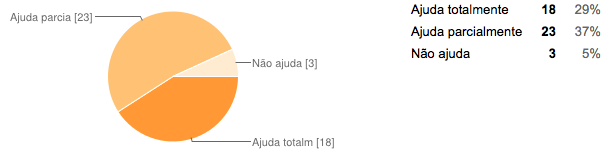
\includegraphics[width=16cm]{images/graficos/questao13.png}
  \caption{Gráfico de resultados da questão 13}
  \label{fig:questao13}
\end{center}
\end{figure}

\textbf{Comentários:}

Uma das grandes motivações para o desenvolvimento deste trabalho foi diminuir o número de pessoas suscetíveis a assaltos, bem como a outros incidentes nos pontos de ônibus. No primeiro capitulo deste trabalho, constatou-se a insatisfação da população no tocante a insegurança existente nos pontos, bem como como que o principal causador dessa insegurança era a falta de informação, sobretudo, sobre o momento que o veículo vai chegar no ponto. 
Isto posto, a questão 13 foi criada com o intuito de validar se o aplicativo ajuda, através da informação disponibilizada e, por conseguinte, do apoio a tomada de decisões fornecido, a diminuir a insegurança, bem como os incidentes que costumeiramente ocorre nos pontos e terminais de ônibus.
O gráfico mostrado na figura \figref{fig:questao13} deixa claro que, para a maioria dos avaliados, a aplicação ajuda de alguma forma a diminuir as ocorrências de delitos nos pontos, onde 29\% afirmaram que a aplicação ajuda totalmente na luta contra insegurança, 37\% consideraram que o sistema ajuda parcialmente, enquanto 5\% acreditaram que a utilização da aplicação não ajuda a diminuir o números de incidentes nos terminais e pontos de ônibus.\newline


\textbf{Questão 14: A forma como é projetada a tarefa de inserir novos incidentes de trânsito lhe motiva a colaborar?}

\begin{center}
\begin{longtable}{c|c|c}
\hline
    \multicolumn{1}{c}{\textbf{Resultado}} & \multicolumn{1}{c}{\textbf{Quantidade}} & \multicolumn{1}{c}{\textbf{Percentual}} \\
\hline
    Sim & 38 &  60\%\\
    \hline
    Não & 6 & 10\%\\
    \hline
\caption{Tabela de resultados obtidos na questão 14}
\label{tabq14}
\end{longtable}
\end{center}


\begin{figure}[h]
\begin{center}
  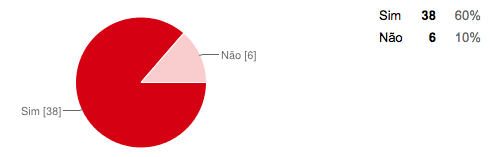
\includegraphics[width=16cm]{images/graficos/questao14.png}
  \caption{Gráfico de resultados da questão 14}
  \label{fig:questao14}
\end{center}
\end{figure}

\textbf{Comentários:}

Um dos pontos chaves da aplicação é a colaboração do usuário com cadastros de ocorrências de incidentes de  trânsito, através destas é possível recomendar as melhores linhas, informar tudo que está acontecendo na cidade, bem como fazer com que os usuários tomem as melhores decisões sobre como, onde e qual ônibus utilizar. Contudo, para que tudo isso aconteça, faz-se necessário que o usuário se sinta motivado a cadastrar uma ocorrência, exatamente como fora discutido no capítulo \ref{ch:crowdsourcing} deste trabalho. Para tanto, esta questão teve como objetivo saber se a forma como a tarefa de cadastrar uma nova ocorrência motiva os usuários a colaborarem com os problemas que estão vivenciando no trânsito.     
	
Os dados revelam que 38 dos 44 avaliados consideraram que a forma como a tarefa de cadastrar novos incidentes foi projetada acaba motivando a colaboração do usuário. Nesse sentido, pode-se afirmar que a maioria dos usuários do aplicativo se sentem motivados a colaborar com a divulgação dos incidentes que estão vivenciando.\newline

\textbf{Questão 15: Depois de receber uma notificação de proximidade do seu ônibus, como você classifica o tempo que você tem para se deslocar para o ponto?}

\begin{center}
\begin{longtable}{c|c|c}
\hline
    \multicolumn{1}{c}{\textbf{Resultado}} & \multicolumn{1}{c}{\textbf{Quantidade}} & \multicolumn{1}{c}{\textbf{Percentual}} \\
\hline
    1 & 1 &  2\%\\
    \hline
    2 & 1 & 2\%\\
    \hline
    3 & 7 &  11\%\\
    \hline
    4 & 28 & 44\%\\
    \hline
    5 & 7 & 7\%\\
    \hline
\caption{Tabela de resultados obtidos na questão 15}
\label{tabq15}
\end{longtable}
\end{center}


\begin{figure}[h]
\begin{center}
  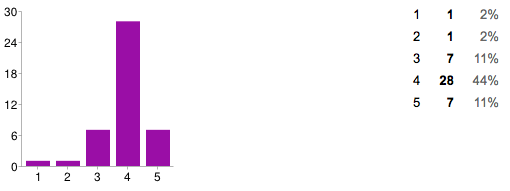
\includegraphics[width=16cm]{images/graficos/questao15.png}
  \caption{Gráfico de resultados da questão 15}
  \label{fig:questao15}
\end{center}
\end{figure}

\textbf{Comentários:}

Uma das funcionalidades do aplicativo é alertar o usuário quando um ônibus de uma linha que costumeiramente este utiliza está se aproximando. Todavia, além de notificar, é necessário que o alerta seja enviando com um tempo de antecedência que permita o usuário conseguir chegar ao ponto antes do ônibus passar. Para avaliar se esse ínterim é satisfatório, bem como se essa funcionalidade realmente funciona como fora especificada, a questão 15 permitiu que o participante da pesquisa classificasse o tempo para se deslocar para o ponto após uma notificação de proximidade com uma nota de 1 a 5, onde 1 significa uma classificação muito ruim e 5 uma avaliação muito boa.
	
Observa-se, no gráfico disponível na figura \figref{fig:questao15}, uma concentração maior na classificação 4, tendo poucas classificações consideras negativas. Assim, sendo possível afirmar que a maioria dos avaliados conseguem se deslocar até o ponto em um tempo hábil.\newline

\textbf{Questão 16: Com a ajuda do aplicativo você consegue saber quais linhas passam em um determinado ponto.}

\begin{center}
\begin{longtable}{c|c|c}
\hline
    \multicolumn{1}{c}{\textbf{Resultado}} & \multicolumn{1}{c}{\textbf{Quantidade}} & \multicolumn{1}{c}{\textbf{Percentual}} \\
\hline
    Concordo totalmente & 25 &  40\%\\
    \hline
    Concordo parcialmente & 17 & 27\%\\
    \hline
     Não concordo & 2 & 3\%\\
    \hline
\caption{Tabela de resultados obtidos na questão 16}
\label{tabq16}
\end{longtable}
\end{center}


\begin{figure}[h]
\begin{center}
  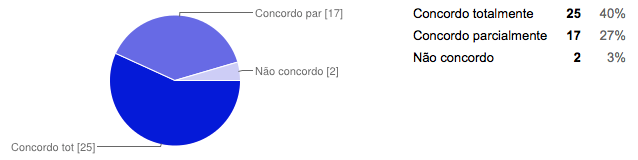
\includegraphics[width=16cm]{images/graficos/questao16.png}
  \caption{Gráfico de resultados da questão 16}
  \label{fig:questao16}
\end{center}
\end{figure}

\textbf{Comentários:}

Outra grande motivação deste trabalho foi melhorar o nível de informação disponível no tocante aos serviços do transporte público. No primeiro capítulo, foi mostrado que a maioria dos usuários de transporte público estão insatisfeitos com a qualidade das informações disponíveis nos terminais de ônibus, sendo uma das principais críticas a dificuldade de saber quais linhas passam por determinado ponto. 

Uma das propostas do aplicativo desenvolvido neste trabalho é informar aos usuários quais linhas passam por um determinado ponto escolhido por este. Todavia, faz-se necessário validar se realmente o sistema funciona como fora especificado. Para tanto, a questão 16 foi criada a fim de questionar aqueles que utilizam frequentemente a aplicação se eles concordam que a mesma consegue fornecer tal serviço.

Observa-se que 42 usuários, de um total de 44, afirmaram concordar com a afirmação feita na questão 16, o que significa dizer que 67\%, dos 70\% dos avaliados que avançaram para fase de avaliação, estão satisfeitos com informação disponibilizada pelo aplicativo no que tange a relação feita entre linhas e pontos de ônibus. \newline

\textbf{Questão 17: De modo geral, como você classifica a usabilidade do aplicativo?}

\begin{center}
\begin{longtable}{c|c|c}
\hline
    \multicolumn{1}{c}{\textbf{Resultado}} & \multicolumn{1}{c}{\textbf{Quantidade}} & \multicolumn{1}{c}{\textbf{Percentual}} \\
\hline
    1 & 3 &  5\%\\
    \hline
    2 & 0 & 0\%\\
    \hline
    3 & 5 &  8\%\\
    \hline
    4 & 30 & 48\%\\
    \hline
    5 & 6 & 10\%\\
    \hline
\caption{Tabela de resultados obtidos na questão 17}
\label{tabq17}
\end{longtable}
\end{center}


\begin{figure}[h]
\begin{center}
  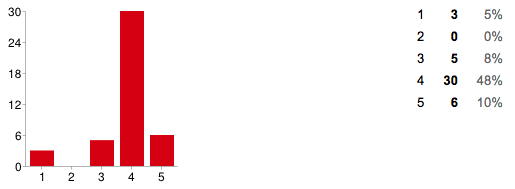
\includegraphics[width=16cm]{images/graficos/questao17.png}
  \caption{Gráfico de resultados da questão 17}
  \label{fig:questao17}
\end{center}
\end{figure}

\textbf{Comentários:}

Umas das grandes preocupações e, sobretudo, um dos requisitos da proposta desenvolvida foi fazer com que a aplicação tivesse uma boa usabilidade, isto é, fosse simples e muito intuitiva, para que, desta forma, pudesse ser utilizada por todos usuários do transporte público. Para tanto, com o objetivo de medir se aplicação realmente atende a proposta, pediu-se aos avaliados que atribuísse uma nota de 1 a 5 para usabilidade do aplicativo, onde 1 significava que o sistema possui uma usabilidade muito ruim, enquanto que uma no 5 significava dizer que a aplicação tem uma usabilidade excelente.
	
Analisando o gráfico presente na figura \figref{fig:questao17}, nota-se a existência de algumas avaliações negativas. Não obstante, observa-se uma concentração bem maior na nota 4, o que acaba mostrando, também, que a maioria dos avaliados não estão totalmente satisfeitos e acreditam que a usabilidade ainda pode melhorar. \newline

\textbf{Questão 18: Você acredita que uma pessoa sem conhecimento técnico utilizaria o FindBus?}


\begin{center}
\begin{longtable}{c|c|c}
\hline
    \multicolumn{1}{c}{\textbf{Resultado}} & \multicolumn{1}{c}{\textbf{Quantidade}} & \multicolumn{1}{c}{\textbf{Percentual}} \\
\hline
    Sim & 41 &  65\%\\
    \hline
    Não & 3 & 5\%\\
    \hline
\caption{Tabela de resultados obtidos na questão 18}
\label{tabq18}
\end{longtable}
\end{center}

\begin{figure}[h]
\begin{center}
  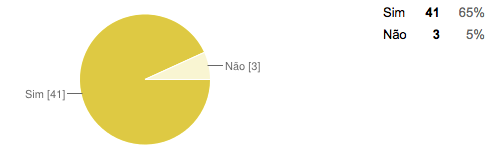
\includegraphics[width=16cm]{images/graficos/questao18.png}
  \caption{Gráfico de resultados da questão 18}
  \label{fig:questao18}
\end{center}
\end{figure}

\textbf{Comentários:}

A questão 18 teve o objetivo de servir como um complemento da questão 17 de modo a contrapor as repostas das duas questões. Para tanto, parte-se da prerrogativa de que se uma pessoa sem nenhum conhecimento técnico consegue utilizar a aplicação, esta possui uma boa usabilidade. Nesse sentido, a questão 18 poderia tanto validar como invalidar o que fora respondido na questão 17.
	
Analisando os dados apresentados na tabela \ref{tabq17}, bem como os dados informados na tabela \ref{tabq18}, nota-se a mesma quantidade de respostas tanto para uma total insatisfação com a usabilidade do aplicativo quanto para não possibilidade de uma pessoa sem conhecimento técnico utilizar o sistema, o que mostra total coerência entre as repostas das duas questões.
	
Nota-se, no gráfico da figura \figref{fig:questao18}, que 65\% dos avaliados, dos 70\% que avançaram para fase de avaliação, afirmaram que mesmo uma pessoa sem conhecimento técnico conseguiria utilizar e usufruir de todos os recursos disponíveis na aplicação.\newline

\textbf{Questão 19: Avalie o FindBus com uma nota de 1 a 5.}


\begin{center}
\begin{longtable}{c|c|c}
\hline
    \multicolumn{1}{c}{\textbf{Resultado}} & \multicolumn{1}{c}{\textbf{Quantidade}} & \multicolumn{1}{c}{\textbf{Percentual}} \\
\hline
    1 & 2 &  3\%\\
    \hline
    2 & 1 & 2\%\\
    \hline
    3 & 3 &  5\%\\
    \hline
    4 & 19 & 30\%\\
    \hline
    5 & 19 & 30\%\\
    \hline
\caption{Tabela de resultados obtidos na questão 19}
\label{tabq19}
\end{longtable}
\end{center}

\begin{figure}[h]
\begin{center}
  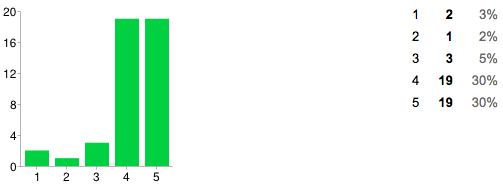
\includegraphics[width=16cm]{images/graficos/questao19.png}
  \caption{Gráfico de resultados da questão 19}
  \label{fig:questao19}
\end{center}
\end{figure}

\textbf{Comentários:}

Por fim, com a finalidade de medir, de modo geral, a satisfação dos usuários com o aplicativo, pediu-se aos avaliados que dessem uma nota de 1 a 5, onde 1 significava uma total insatisfação e 5 uma total satisfação com o sistema. 
	
O gráfico mostrado na figura \figref{fig:questao19}, aponta uma grande concentração nas respostas 4 e 5, onde 19 avaliados atribuíram uma no 4 e 19 atribuíram uma nota 5, o que significa dizer que 38 usuários, dos 44 avaliados, estão satisfeitos com o uso do aplicativo.\newline

\section{Análise dos resultados}
\label{sc:analiseResultados}

A partir dos dados, bem como das analises parciais apresentadas na seção \ref{sc:apresentacaoResultados}. deste trabalho podemos concluir que, para o grupo avaliado, o aplicativo conseguiu cumprir com os objetivos gerais propostos na seção \ref{sc:objetivoGerais}, haja vista que a maioria dos usuários que participaram da pesquisa apresentaram respostas positivas em relação a utilização do aplicativo e, sobretudo, as informações fornecidas pelas principais funcionalidades deste.
	
Observa-se, através das respostas coletadas nas questões  2, 4, 6 e 7, que o aplicativo realmente consegue fazer com que os usuários visualizem, a priori, somente as informações no tocante ao transporte público e mobilidade de sua cidade, sendo, portanto, encaixado no contexto da cidade onde ele se encontra, conforme fora proposto no primeiro objetivo específico deste trabalho. 
	
Nota-se, também, analisando os dados apresentados na questão 14, que a forma como a tarefa de inserir novos incidentes de trânsito acaba estimulando a colaboração do usuário, visto que a maioria dos avaliados afirmaram sentirem-se motivados a colaborar com a divulgação dos problemas enfrentados durante o dia-a-dia da cidade. Isto posto, pode-se afirmar que segundo objetivo específico proposto neste trabalho também conseguiu ser atingido com o desenvolvimento da proposta.
	
Ademais, de acordo com os dados mostrados nas questões 4, 5, 10, 12 e 13, pode-se afirmar que o aplicativo consegue realmente fazer com que seus usuários saibam a real localização de um determinado ônibus juntamente com informações de distâncias e linhas, podendo, desta forma, prever o exato momento que o ônibus passará em um determinado ponto e, por conseguinte, otimizar seu temo e ficar menos vulnerável a insegurança existente no pontos e terminais, exatamente como proposto no terceiro objetivo específico deste trabalho. 

De modo a comprovar que o quarto objetivo específico deste trabalho foi atendido com o desenvolvimento da proposta, os dados da coletados na questão 11 foram analisados. Os dados mostram que a maioria dos avaliados consideraram o tempo de atualização e localização dos ônibus aceitável, sendo possível monitorar o deslocamento do veículo em, praticamente, tempo real.
	
O quinto objetivo específico deste trabalho propusera que a proposta permitisse que o usuário visualizasse todas as rotas, linhas e pontos de ônibus da cidade onde ele se encontra, bem como saber quais linhas passam por um determinado ponto. Analisando os dados obtidos nas questões 6 e 16, observa-se uma grande quantidade de respostas positivas e, desta forma, apoiando-se nas analises parciais apresentadas nessas duas questões, pode-se afirmar que o aplicativo realmente consegue cumprir o objetivo proposto.
	
Outrossim, os dados coletados na questão 7, bem como a analise parcial feita no comentário da referida questão, mostram que os usuários conseguem cadastrar ocorrências de trânsito por eles vivenciadas, bem como visualizar as ocorrências cadastradas por outros usuários, validando, assim, o sexto e sétimo objetivos específicos apresentados na seção \ref{sc:objetivoEspecificos} deste trabalho.  
	
O oitavo objetivo específico deste trabalho propusera que a proposta desenvolvida fosse capaz de recomendar a melhor rota para que o usuário chegue ao seu destino. Assim sendo, as respostas obtidas nas questões 8 e 9, de acordo com a analise parcial realizada nessas questões, que mostra a discrepância existente entre o número de respostas positivas em relação as negativas, pode-se afirmar que aplicativo consegue, apoiando-se nas informações disponibilizadas pelos próprios usuários através da colaboração, recomendar as melhores linhas para que o usuário consiga chegar a um determinado destino.

	





